\documentclass[border=10pt]{standalone}
\usepackage{tikz}
\usetikzlibrary{arrows.meta, positioning, shapes.geometric, calc}

\begin{document}
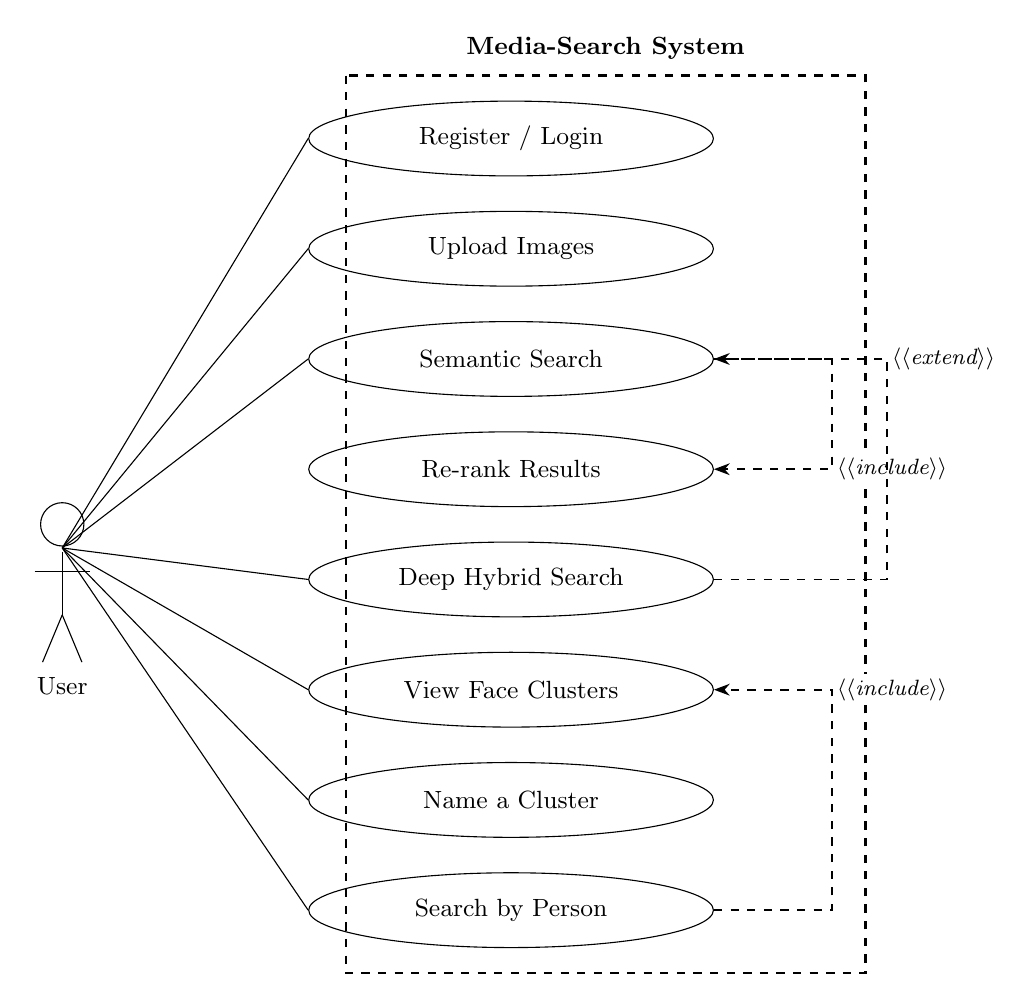
\begin{tikzpicture}[
  uc/.style={draw, ellipse, text width=3.4cm, minimum height=0.95cm,
             align=center, font=\small},
  rel/.style={->, >=Stealth, dashed, semithick},
  lbl/.style={font=\footnotesize\itshape, fill=white, inner sep=1.5pt},
]

%% ---- Actor (stick figure) ----
\node[draw, circle, minimum size=0.55cm, fill=white] (head) at (-1.2, 0.3) {};
\draw (-1.2,-0.05) -- (-1.2,-0.85);
\draw (-1.55,-0.3) -- (-0.85,-0.3);
\draw (-1.2,-0.85) -- (-1.45,-1.45);
\draw (-1.2,-0.85) -- (-0.95,-1.45);
\node[font=\small] at (-1.2,-1.75) {User};

%% ---- Use Cases ----
\node[uc] (reg)    at (4.5,  5.2) {Register / Login};
\node[uc] (upload) at (4.5,  3.8) {Upload Images};
\node[uc] (search) at (4.5,  2.4) {Semantic Search};
\node[uc] (rerank) at (4.5,  1.0) {Re-rank Results};
\node[uc] (deep)   at (4.5, -0.4) {Deep Hybrid Search};
\node[uc] (fclust) at (4.5, -1.8) {View Face Clusters};
\node[uc] (fname)  at (4.5, -3.2) {Name a Cluster};
\node[uc] (fsrch)  at (4.5, -4.6) {Search by Person};

%% ---- Association lines (actor -> use cases) ----
\foreach \t in {reg, upload, search, deep, fclust, fname, fsrch}
  \draw (-1.2,0.0) -- (\t.west);

%% ---- System boundary ----
\draw[dashed, thick] (2.4, 6.0) rectangle (9.0, -5.4);
\node[font=\small\bfseries] at (5.7, 6.35) {Media-Search System};

%% ---- Relationships (positioned to the RIGHT of ellipses, no overlap) ----
%% search <<include>> rerank  (arrow goes right side, outside ellipse)
\draw[rel] (search.east) -- ++(1.5,0) |- node[lbl, right]{$\langle\langle$include$\rangle\rangle$} (rerank.east);

%% deep <<extend>> search  (right side)
\draw[rel] (deep.east) -- ++(2.2,0) |- node[lbl, right]{$\langle\langle$extend$\rangle\rangle$} (search.east);

%% fsrch <<include>> fclust (right side)
\draw[rel] (fsrch.east) -- ++(1.5,0) |- node[lbl, right]{$\langle\langle$include$\rangle\rangle$} (fclust.east);

\end{tikzpicture}
\end{document}
